\section{Results and Tests}

\subsection{Energy optimization}
During this assignment we have employed several methods for decreasing the power consumption of the program. We have focused on power consumption of both when the program idle and active. The eAprofiler in the simplicity studio bundle has been used to analyze the power consumption at various stages in the program. For completeness both the power consumptions before and after the an optimization is illustrated.


\subsubsection{Idle}
When the program is idle the power consumption is reduced. The energy optimized program should consume   significantly less energy. The high frequency peripheral is turned off, the low energy oscillator is turned off and the DAC is partly turned off. The DAC is not completely disabled and will consume some power. The CPU remain in deep sleep during this time. The output from the eAprofiler for the energy optimized program can be seen in figure 3 for comparison the non optimized program can be seen in figure 4. 


\begin{figure}[H]
  \centering
  % Trim er [left bottom right top]
  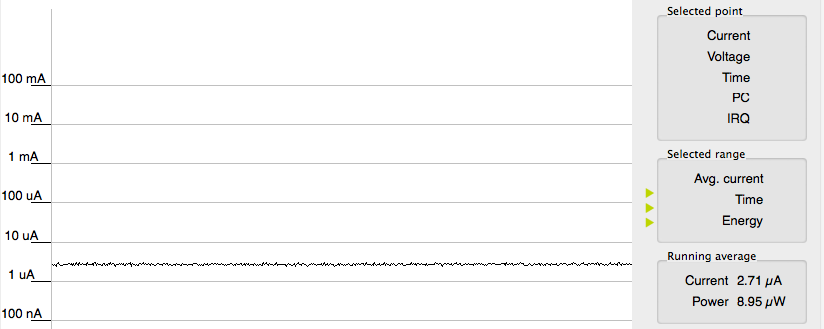
\includegraphics[clip, trim=0cm 0cm 0cm 0cm, width=12cm]{fig/idleEnergy.png}
  \caption{Low energy timer in idle mode}
\end{figure}

\begin{figure}[H]
  \centering
  % Trim er [left bottom right top]
  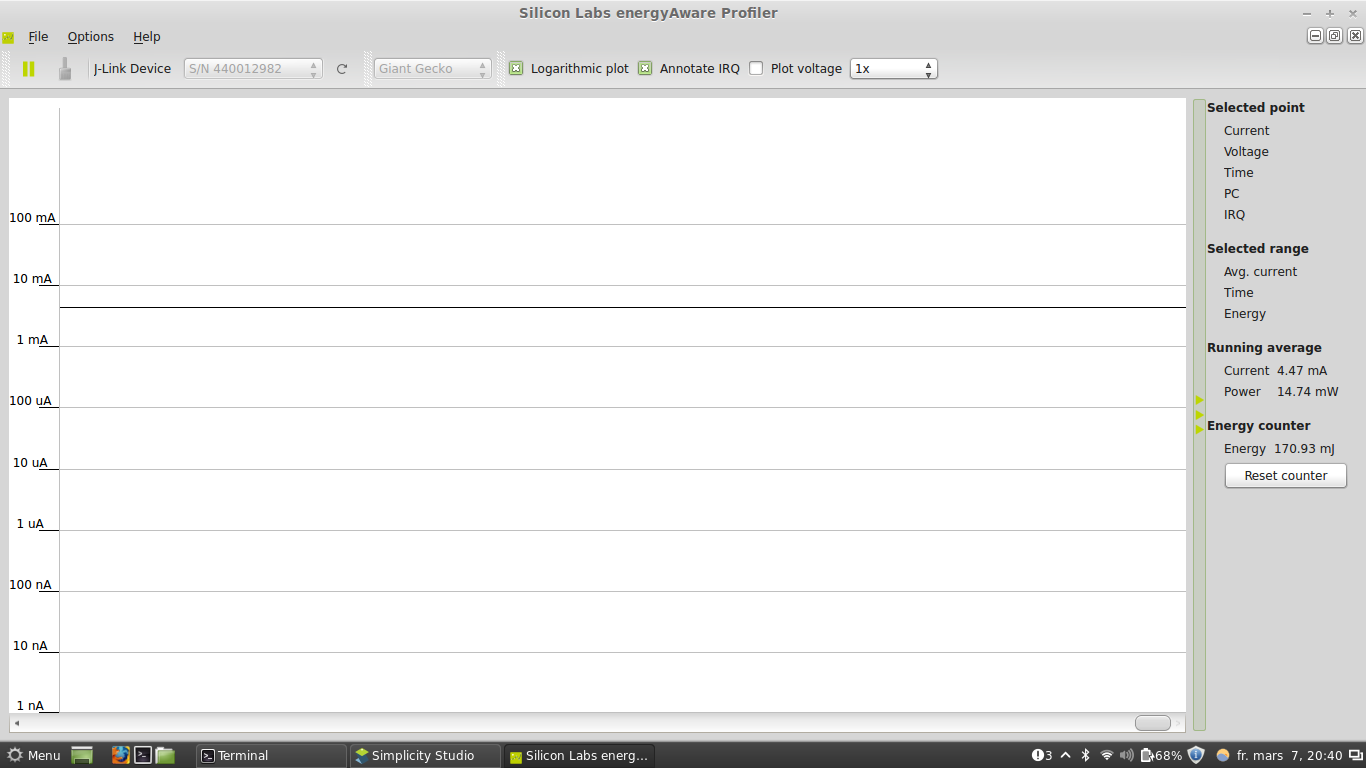
\includegraphics[clip, trim=0cm 0cm 0cm 0cm, width=12cm]{fig/Timer1Idle.png}
  \caption{Regular timer in idle mode}
\end{figure}


As seen the the energy usage is set at an comfortable level of 74 micro amperes. This is significantly less than before the optimization, where the idle processor consume 4.5 milli amperes.  




\subsubsection{Running}
During the running of the program the CPU and the DAC is not utilised every clock cycle. It is possible to exploit this by entering deep sleep when the processor is not active and configure the DAC stop/hold mode. Also, further energy consumption should be reduced by using the low energy timer. It is not necessary to power the CPU and the DAC when not used. This can significantly reduce the power consumption when the program is active as illustrated in the figures below. The first figure illustrates the energy when using deepsleep and stop/hold mode for the DAC. The second figure illustrates the power consumption when no optimizations techniques are in use.

\begin{figure}[H]
  \centering
  % Trim er [left bottom right top]
  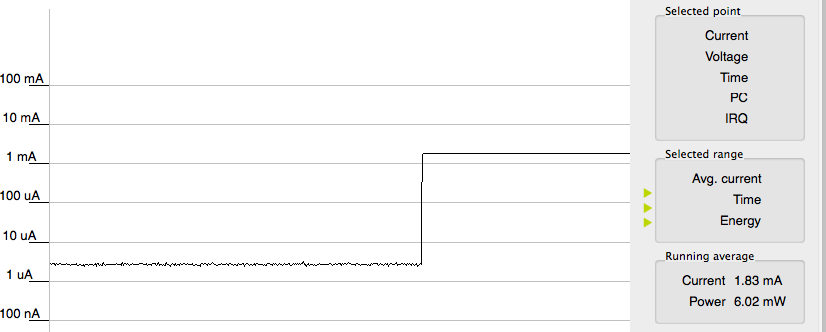
\includegraphics[clip, trim=0cm 0cm 0cm 0cm, width=12cm]{fig/marioEnergy.png}
  \caption{Low energy timer while running}
\end{figure}



As seen by comparing the figures, the gains are significant when turning off the components during idle cycles. 


\subsection{Sounds functionality}


\subsubsection{Sound effects}


\subsubsection{Music}


